% Propósito: comparar la separación espacial de razones en una escala lineal
% con la separación uniforme de sus logaritmos.
% Origen: L_Q=10 log10(Q/Q0), para Q/Q0=1,10,100,1000.
% Descripción accesible: en una escala lineal de cero a mil, las razones 1 y 10
% quedan casi superpuestas cerca del origen y 100 permanece en la primera
% décima parte. En la representación logarítmica, 1, 10, 100 y 1000 quedan
% igualmente espaciados y corresponden a 0, 10, 20 y 30 dB.
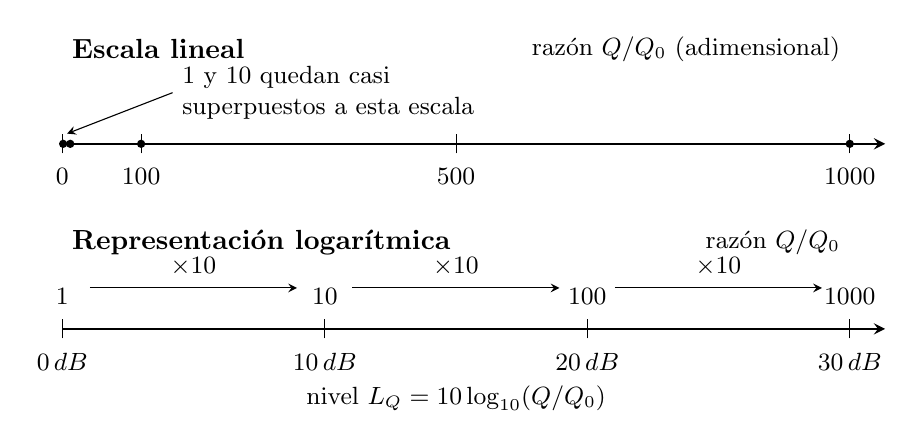
\begin{tikzpicture}[font=\small,>=stealth,x=1cm,y=1cm]
    % Escala lineal: encabezado, anotación y eje ocupan bandas distintas.
    \node[anchor=west,font=\bfseries] at (0,3.25) {Escala lineal};
    \node[anchor=east] at (10,3.25)
        {razón \(Q/Q_0\) (adimensional)};
    \draw[->,thick] (0,2.05) -- (10.45,2.05);
    \foreach \x/\etiqueta in {0/0,1/100,5/500,10/1000}{
        \draw (\x,1.93) -- (\x,2.17);
        \node[below=2pt] at (\x,1.93) {\etiqueta};
    }
    \fill (0.01,2.05) circle (1.5pt);
    \fill (0.1,2.05) circle (1.5pt);
    \fill (1,2.05) circle (1.5pt);
    \fill (10,2.05) circle (1.5pt);
    \node[anchor=west,align=left] (anotacion) at (1.40,2.70)
        {\(1\) y \(10\) quedan casi\\superpuestos a esta escala};
    \draw[->] (anotacion.west) -- (0.06,2.18);

    % Representación logarítmica: las razones, los niveles y los factores
    % multiplicativos se colocan en franjas verticales independientes.
    \node[anchor=west,font=\bfseries] at (0,0.80)
        {Representación logarítmica};
    \node[anchor=east] at (10,0.80) {razón \(Q/Q_0\)};
    \draw[->,thick] (0,-0.30) -- (10.45,-0.30);
    \foreach \x/\razon/\nivel in {
        0/1/0,
        3.333/10/10,
        6.666/100/20,
        10/1000/30
    }{
        \draw (\x,-0.42) -- (\x,-0.18);
        \node[above=2pt] at (\x,-0.18) {\(\razon\)};
        \node[below=2pt] at (\x,-0.42) {\(\nivel\,\text{dB}\)};
    }
    \node at (5,-1.18) {nivel \(L_Q=10\log_{10}(Q/Q_0)\)};

    \foreach \x in {0,3.333,6.666}{
        \draw[->] (\x+0.35,0.22) -- (\x+2.98,0.22)
            node[midway,above=1pt]{\(\times10\)};
    }
\end{tikzpicture}
